\documentclass[a4paper]{report}
\usepackage[utf8]{inputenc}
\usepackage[T1]{fontenc}
\usepackage[francais]{babel}
%\frenchbsetup{StandardLists=true} % à inclure si on utilise \usepackage[french]{babel}
\usepackage{enumitem}
\usepackage{amssymb}
\usepackage{graphicx}
\usepackage{fullpage}
\usepackage{eso-pic}
\usepackage{listings}
\newcommand{\HRule}{\rule{\linewidth}{0.5mm}}
\newcommand{\blap}[1]{\vbox to 0pt{#1\vss}}
\newcommand\AtUpperLeftCorner[3]{%
  \put(\LenToUnit{#1},\LenToUnit{\dimexpr\paperheight-#2}){\blap{#3}}%
}

\title{\LARGE{snake }}
\author{Ait el djoudi Karim \\ janvier 16, 2019}
\date{\today}%il veux pas s'afficher 
\makeatletter

\begin{document}
 
\begin{titlepage}
    \enlargethispage{2cm}
 \vfill
    \AddToShipoutPicture{\AtUpperLeftCorner{1.5cm}{1cm}{
\includegraphics[width=9.5cm]{pr.jpg}}}
\vfill
    \begin{center}
        \vspace*{10cm}
 
        \textsc{\@title}
        \HRule
        \vspace*{0.5cm}
 
        \large{\@author} 
    \end{center}
 
    \vspace*{5cm}
 
    \begin{center}
        \makebox[\textwidth]{
\includegraphics[width=13.5cm]{snake.jpg}}
    \end{center}
 \end{titlepage}
\ClearShipoutPicture
\newpage
\chapter*{snake.}
\section{Enoncé}

Le but de dans ce jeu, on contrôle un serpent avec lesflèches du clavier.\\ Pour gagner, le serpent doit manger un max de point pour evoluer le score du jeux .\\ On perd si le serpent sort de la fenˆetre ou s’il se mord la queue.\\

\section{Fichiers et Méthodes}
\begin{onehalfspace}
\begin{description}
\item[Classe Point.java :\\] cette classe elle contien \\ un constructeur de point x et y et une méthode boolean qui verfier si c'est point ou pas et une méthodes ToString pour l'affichage.\\
\end{description}
\end{onehalfspace}
\begin{onehalfspace}
\begin{description}
\item[Classe Snake.java :\\] cette classe je commence a créér mon serpent (addition point de la longueur max 3) et je le donne des couleur unique exmple (mon serpent ayent une couleur de debut ORANGE puis a sa morte ROUGE)   : \\
\end{description}
\end{onehalfspace}

\begin{onehalfspace}
\begin{description}
\item[Classe Painter.java :\\] cette classe je dessine les foremes et les couleurs et aussi la couleur du point a manger change a chaque fois et aussi le serpent change de coleur selon le point a manger c'est plus agreable et j'affiche le  Niveau et le Score de jeux et en cas de perd j'affiche le message "Game Over","Appuyez sur Entrée pour rejoué ou Echape pour quitte"\\

\end{description}
\end{onehalfspace}

\begin{onehalfspace}
\begin{description}
\item[Classe Grid.java :\\] cette classe je génère les les couleur des point et leur postion aleatoirement dans la grille. \\

\end{description}
\end{onehalfspace}

\begin{onehalfspace} 
\begin{description}
\item[Classe Gameloop.java :\\] cette classe je génère le vitesse de jeux et le temp plus des methodes de debut de jeux(isKeyPressed()) et fin (pause()) . \\
\end{description}
\end{onehalfspace}


\begin{onehalfspace}
\begin{description}
\item[Classe Main.java :\\] cette classe je génère le menu d'entre(iterface graphique j'ai mis une photo deux bouton star et exit et j'ai afficher aussi mon prenom ) et la grille de jeux puis les methodes: \\
\textbf{handle} debut de jeux et avec des manipulation clavier haut gauche bas droit et en cas de perd en peux rejouer ou bien fermer le jeu . \\ 
\end{description}
\end{onehalfspace}

\section{Problèmes}
\begin{onehalfspace} 
\begin{description}
L'algorithm il Fonction trés bien mais j'avais un petit point qui foction pas quand j'ai mon serpent au debut avant de mange le premie point quand je clique sur deux bouton de clavier gauche et bas en même temp ou droit et bas ou gauche et haut ou droit et haut le serpent il fait demi-tour (marche arrière) mais dès que je mange un point et j'essaye de faire cette expérience le serpent tourne mais il mort direct j'arrive pas a corriger ce problème. a part ca il fonction trés bien.\\
\end{description}
\end{onehalfspace}
\begin{onehalfspace} 
\begin{description}
\begin{center}
 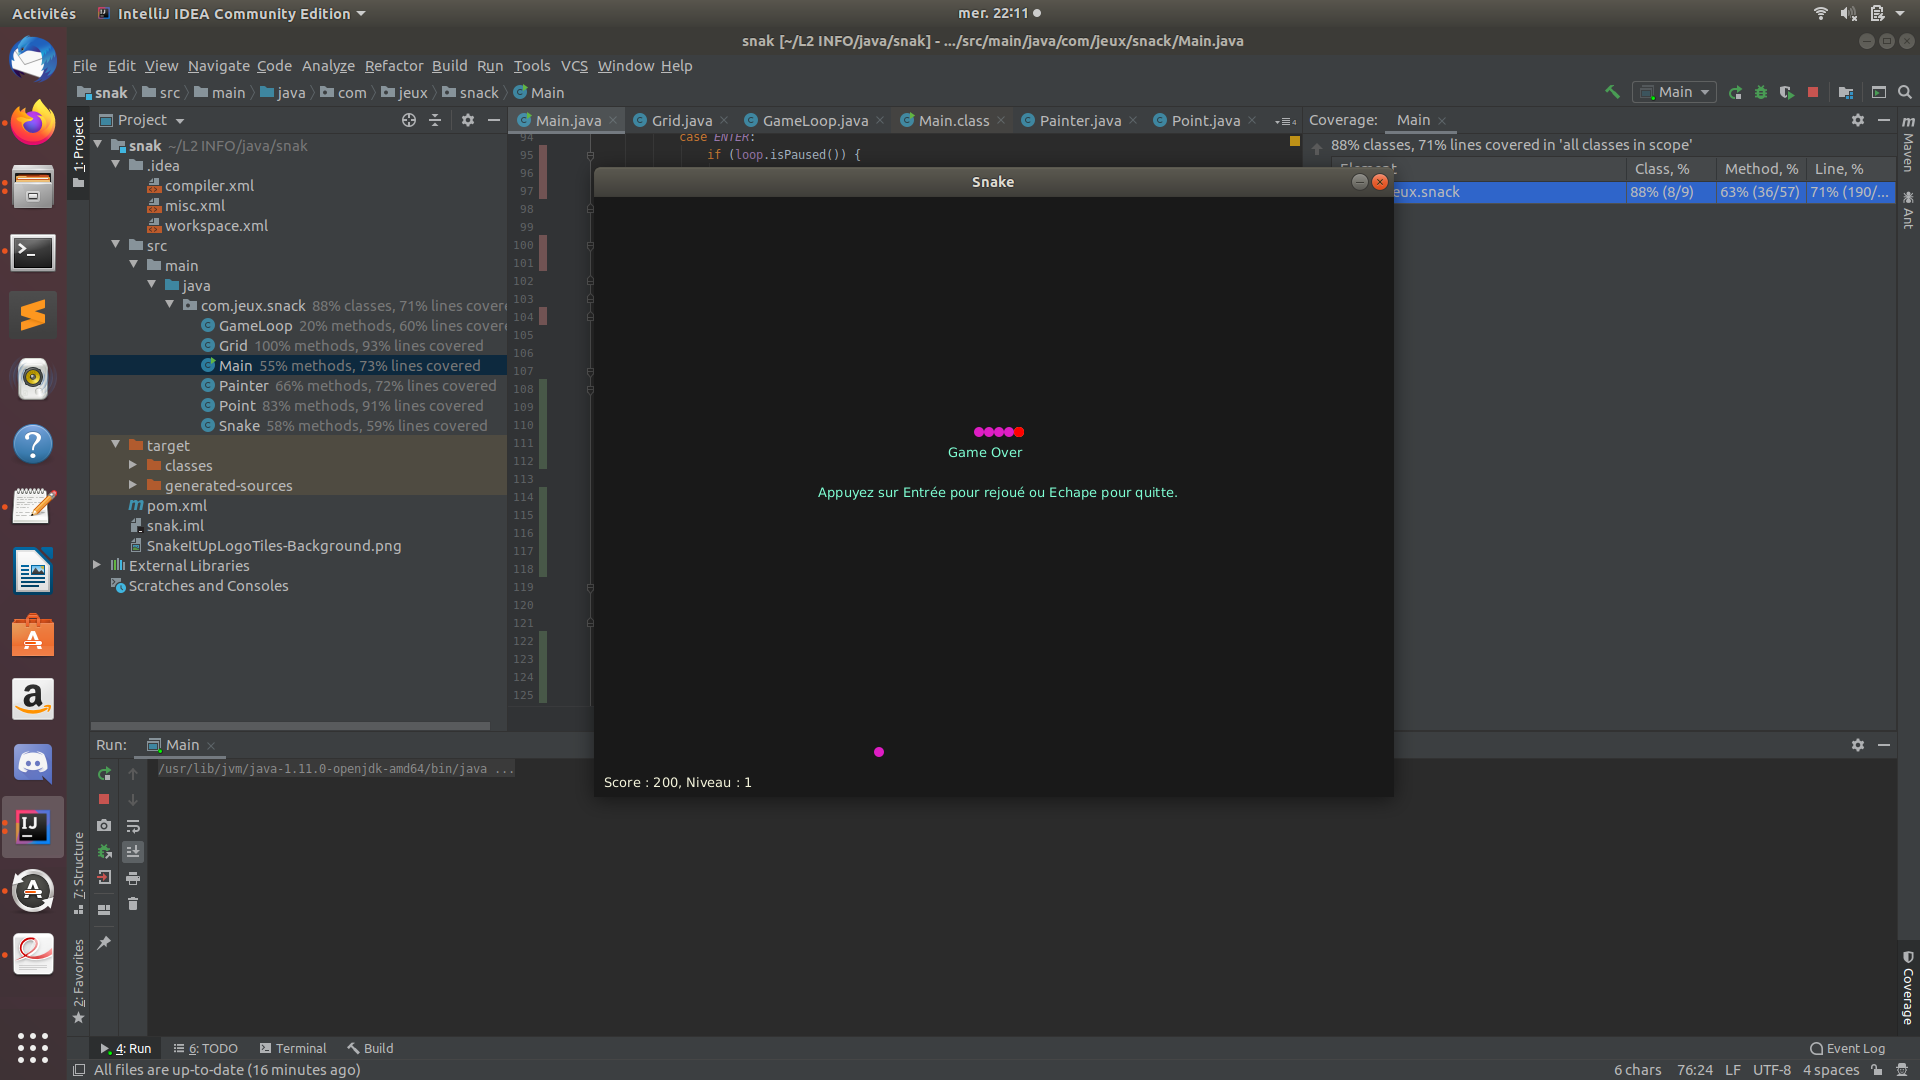
\includegraphics[width=13.5cm]{exp.png}
\end{center}
\end{description}
\end{onehalfspace}

\section{Exemple utilisation}
\begin{onehalfspace} 
\begin{description}
\begin{center}
     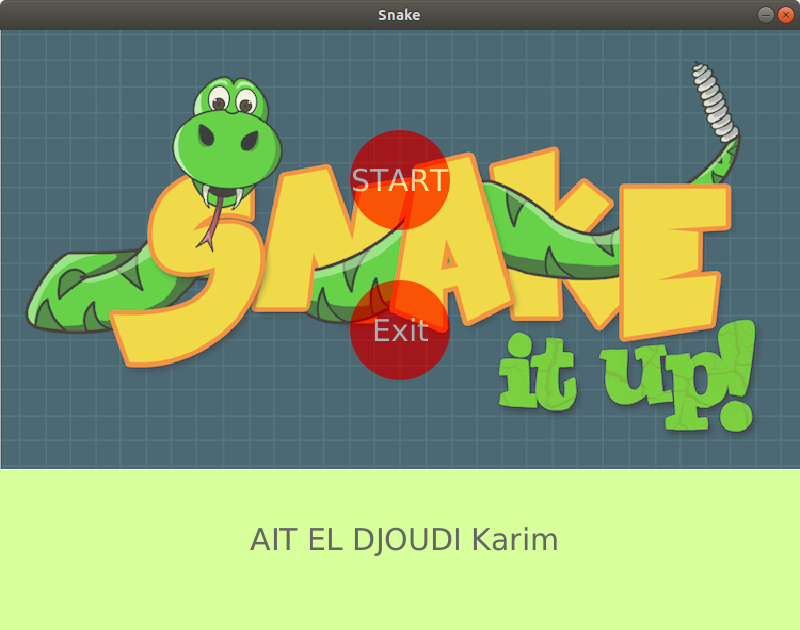
\includegraphics[width=13.5cm]{ex.png}
\end{center}
\end{description}
\end{onehalfspace}
\begin{onehalfspace} 
\begin{description}
\begin{center}
     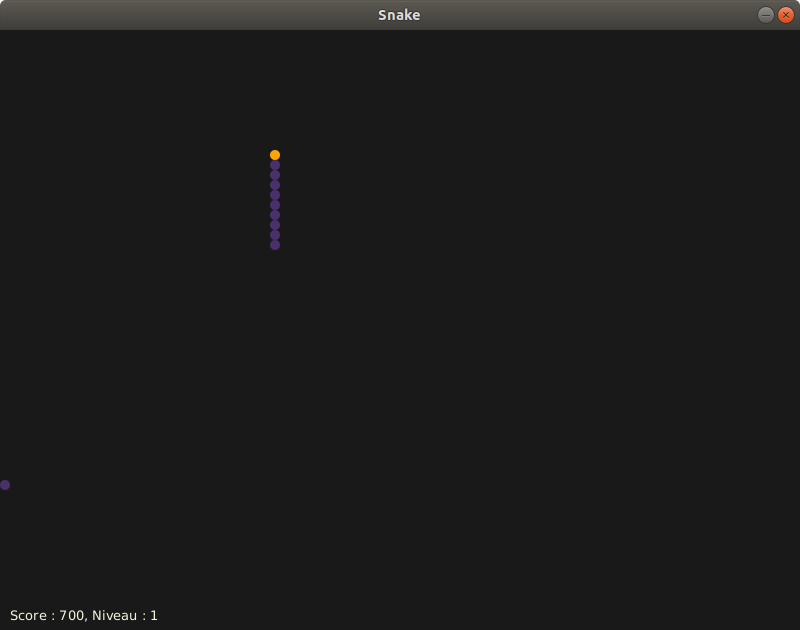
\includegraphics[width=13.5cm]{exp1.png}
\end{center}
\end{description}
\end{onehalfspace} 

\begin{onehalfspace} 
\begin{description}
\begin{center}
     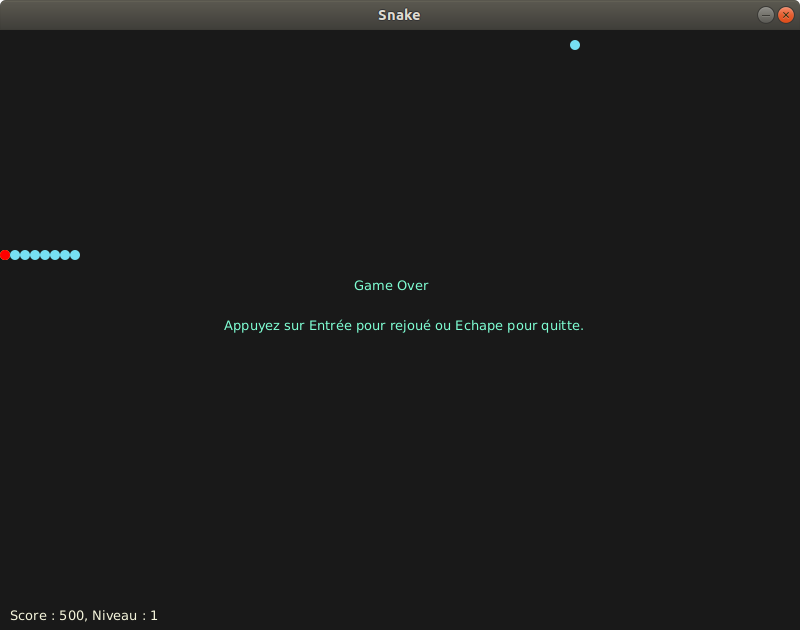
\includegraphics[width=13.5cm]{exp2.png}
\end{center}
\end{description}
\end{onehalfspace} 
\end{document}
